%%
%% 章:グラフィック
%%------------------------------------------------------------------------------------------------------------------------------%%
\chapter{グラフィック}
\LaTeX{}文書の中に写真や、他のツールで描いた図などを挿入することができる。
昔は\LaTeX{}に図を挿入するといえば EPS 形式がほとんどだったが、今日では PDF 形式(ラスター画像なら JPEG や PNG 形式)で挿入する方が速くトラブルもない。\\

逆に、\LaTeX{}で組んだ文章や数式などを、他のソフトに PDF などのベクトル形式で挿入するすることも可能である。
文字を変形したり、文字や背景に色を付けたりする方法も本章で扱う。
%%
%% 節:LaTeX と図
%%--------------------------------------------------------------------------------------------------------------------%%
\section{\LaTeX{}と図}
\LaTeX{}だけで図を描く方法は多数存在する。
いくつか例を挙げる。
\vspc{-0.50zw}\begin{itemize}\setlength{\leftskip}{-1.00zw}%\setlength{\labelsep}{+1.00zw}
\item \LaTeX{}標準の pictuer 環境(現在は推奨しない)。
\item pict2e パッケージの picture 環境。
\item PostScript ベースの PSTricks というパッケージ群(PDF ベースのワークフローでは推奨しない)。
\item T\textit{i}kZ
\item 大熊一弘{\small 氏}の emath パッケージ。
\end{itemize}\vspc{-0.50zw}
これらは全てコマンド(文字による命令)で図を描くため、人によっては敷居が高いと感じるかもしれない。\\

より簡単な方法として、Adobe Illustrator や Inkscape などのドローツール、PowerPoint や Keynote などのスライド作成ソフト、Excel や R などの統計グラフ機能を持ったソフトを活用して図を描き、PDF 形式で保存して\LaTeX{}文書に挿入することができる。
複雑な表も Excel で組んで PDF で保存することで、同様に挿入することができる(Excel の図表が美しいかどうかは別問題だが)。\\

デジカメで撮影した写真やスキャン画像、Windows のペイントや GIMP、Photoshop などで描いた画像は、JPEG や PNG 形式のままで挿入することができる。
%%
%% 節:LaTeX での図の読み込み方
%%--------------------------------------------------------------------------------------------------------------------%%
\section{\LaTeX{}での図の読み込み方}
\LaTeX{}文書への図の挿入方法は、ワークフロー(処理の流れ)によって少しずつ異なる。\enlargethispage{+1.00zw}
本稿で主に取り扱っている日本語の PDF ワークフローでは dvipdfmx が中心になるが、ここでは全てに共通のことを説明する。\\

グラフィックを扱うためには、プリアンブルで次のように graphicx パッケージを読み込み、本文中は \verb`\includegraphics` コマンドを用いて図を挿入する。
\vspc{+0.50zw}\begin{mdframed}[roundcorner=0.50zw,leftmargin=3.00zw,rightmargin=3.00zw,skipabove=0.40zw,skipbelow=0.40zw,innertopmargin=4.00pt,innerbottommargin=4.00pt,innerleftmargin=5.00pt,innerrightmargin=5.00pt,linecolor=gray!020,linewidth=0.50pt,backgroundcolor=gray!20]
\verb`\documentclass[`\texttt{\textcolor{blue}{ドライバ名}}\verb`]{jsarticle}`                                      \\
\verb`\usepackage[hiresbb]{graphicx}`                                                                               \\
\verb`\begin{document}`                                                                                             \\
\verb`(……本文……)`                                                                                             \\
\verb`\includegraphics[`\texttt{\textcolor{blue}{オプション}}\verb`]{`\texttt{\textcolor{blue}{ファイル名}}\verb`}` \\
\verb`(……本文……)`                                                                                             \\
\verb`\end{document}`
\end{mdframed}\vspc{-0.70zw}
この\texttt{\textcolor{blue}{ドライバ名}}のところに dvipdfmx、pdftex、xetex、luatex などが入る。
\texttt{\textcolor{blue}{オプション}}には \verb`[width=5cm]` や \verb`[height=3cm]` のような挿入枠の大きさの指定などが入る。\\

以下では、ドライバ毎に更に詳述する。
%%
%% 項:dvipdfmx の場合
%%----------------------------------------------------------------------------------------------------------%%
\subsection{dvipdfmx の場合}
dvipdfmx は p\TeX、up\TeX{}で標準的に使われるドライバである。
PDF、PNG、JPEG 形式の図が扱えるほか、Ghostscript の力を借りて EPS 形式の図も扱うことができる。
\vspc{+0.50zw}\begin{mdframed}[roundcorner=0.50zw,leftmargin=3.00zw,rightmargin=3.00zw,skipabove=0.40zw,skipbelow=0.40zw,innertopmargin=4.00pt,innerbottommargin=4.00pt,innerleftmargin=5.00pt,innerrightmargin=5.00pt,linecolor=gray!020,linewidth=0.50pt,backgroundcolor=gray!20]
\verb`\documentclass[dvipdfmx]{jsarticle}`     \\
\verb`\usepackage[hiresbb]{graphicx}`          \\
\verb`\begin{document}`                        \\
\verb`\includegraphics[width=5cm]{sample.pdf}` \\
\verb`\end{document}`
\end{mdframed}\vspc{-0.70zw}
これを p\LaTeX{}と dvipdfmx で処理して PDF を作成する。
%%
%% 項:dvips の場合
%%----------------------------------------------------------------------------------------------------------%%
\subsection{dvips の場合}
PDF ではなく PostScript 出力が必要な場合に使うドライバである。
扱える図は EPS 形式のみである。
EPS 形式の図をそのまま取り込むだけなので、Ghostscript などを必要としない。\\

dvips を使う場合は \verb`\documentclass[dvips]{jsarticle}` とする。
%%
%% 項:pdfTeX、XeTeX、LuaTeX の場合
%%----------------------------------------------------------------------------------------------------------%%
\subsection{\pdfTeX、X\raisebox{-1.60pt}{{$\exists$}}\hspc{-1.00pt}\TeX、\LuaTeX{}の場合}
これらのエンジンは PDF を自前で出力することができる。
クラフィックオプションはそれぞれ pdftex、xetex、luatex である。
PDF、JPEG、PNG、JBIG2 の他、\MP{}の出力する単純な EPS ファイル(MPS ファイル)にも対応している。
一般の EPS ファイルは Ghostscript で PDF に変換してから取り込む。
%%
%% 節:graphicx パッケージの詳細
%%--------------------------------------------------------------------------------------------------------------------%%
\section{graphicx パッケージの詳細}
ここまでに何度か \verb`\usepackage[`\texttt{\textcolor{blue}{オプション}}\verb`]{graphicx}` のような書き方が出てきたので、ここで少しまとめてみる。\\
オプションの部分に記述することができる主なものには、以下のものがある。
\vspc{-0.50zw}\begin{itemize}\setlength{\leftskip}{8.00zw}\setlength{\labelsep}{+1.00zw}
\item [\texttt{draft~~~~~~~~~}] 図を表示しない(枠とファイル名のみ表示する)。
\item [\texttt{final~~~~~~~~~}] 図を表示する(デフォルト)。
\item [\texttt{hiresbb~~~~~~~}] EPS または xbb ファイルに含まれる高解像度バウンディングボックス(HiResBoundingBox)情報を利用する。
\item [\texttt{nosetpageesize}] PDF ファイルのページサイズを自動設定しない(\TeX\ Live 2016 以降)。
\end{itemize}\vspc{-0.50zw}
draft と hiresbb は個々の図に対しても指定することができる。
通常は final オプションは不要だが、次のような場合に便利である。
\vspc{+0.50zw}\begin{mdframed}[roundcorner=0.50zw,leftmargin=3.00zw,rightmargin=3.00zw,skipabove=0.40zw,skipbelow=0.40zw,innertopmargin=4.00pt,innerbottommargin=4.00pt,innerleftmargin=5.00pt,innerrightmargin=5.00pt,linecolor=gray!020,linewidth=0.50pt,backgroundcolor=gray!20]
\begin{verbatim}
\documentclass[dvipdfmx,draft]{jsarticle} % 全体はドラフトモードで
\usepackage[final]{graphicx}              % 図はちゃんと表示する
\end{verbatim}
\end{mdframed}\vspc{-0.70zw}
graphicx パッケージを使えば、図を取り込むための \verb`\includegraphics` 以外にも、図や文字を回転・拡大・縮小する命令が使用可能となる(後述)。
%%
%% 節:\includegraphics の詳細
%%--------------------------------------------------------------------------------------------------------------------%%
\section{$\backslash$includegraphics の詳細}
例えば、\enlargethispage{+1.40zw}
\vspc{+0.50zw}\begin{mdframed}[roundcorner=0.50zw,leftmargin=3.00zw,rightmargin=3.00zw,skipabove=0.40zw,skipbelow=0.40zw,innertopmargin=4.00pt,innerbottommargin=4.00pt,innerleftmargin=5.00pt,innerrightmargin=5.00pt,linecolor=gray!020,linewidth=0.50pt,backgroundcolor=gray!20]
\begin{verbatim}
\includegraphics[width=3cm]{tiger.pdf}
\end{verbatim}
\end{mdframed}\vspc{-0.70zw}
とすると、tiger.pdf という画像を 3\,cm 幅で取り込んで、その場所に出力(表示)する。
画像は 1 つの大きな文字として扱われるので、必要に応じて center 環境などに入れておく。\\

画像ファイルは通常、文書ファイルと同じフォルダに置いておくが、例えばサブフォルダ sub1、sub2 の中の図も探させたい場合は、
\vspc{+0.50zw}\begin{mdframed}[roundcorner=0.50zw,leftmargin=3.00zw,rightmargin=3.00zw,skipabove=0.40zw,skipbelow=0.40zw,innertopmargin=4.00pt,innerbottommargin=4.00pt,innerleftmargin=5.00pt,innerrightmargin=5.00pt,linecolor=gray!020,linewidth=0.50pt,backgroundcolor=gray!20]
\begin{verbatim}
\graphicspath{{sub1/}{sub2/}}
\end{verbatim}
\end{mdframed}\vspc{-0.70zw}
という命令を書いておく。
その他、\LaTeX{}の入力ファイルを見つけられるところなら、どこに図を置いても構わない。
次のようにパスを指定することもできる。
\vspc{+0.50zw}\begin{mdframed}[roundcorner=0.50zw,leftmargin=3.00zw,rightmargin=3.00zw,skipabove=0.40zw,skipbelow=0.40zw,innertopmargin=4.00pt,innerbottommargin=4.00pt,innerleftmargin=5.00pt,innerrightmargin=5.00pt,linecolor=gray!020,linewidth=0.50pt,backgroundcolor=gray!20]
\begin{verbatim}
\includegraphics[width=5cm]{C:/picture/flowers.jpg}
\end{verbatim}
\end{mdframed}\vspc{-0.70zw}
パスの区切りは Windows 環境でも \verb`\` や \textyen{}ではなく \verb`/` を用いる。\\

\verb`\includegraphics` は次のオプションを理解する。
\vspc{-0.50zw}\begin{itemize}\setlength{\leftskip}{-1.00zw}%\setlength{\labelsep}{+1.00zw}
\item width は幅を指定する。上の例では画像の幅を 5\,cm にスケール(拡大または縮小)して出力している。
\item height は高さを指定する。
  \begin{quote}
    \verb'\includegraphics[height=3cm]{...}'
  \end{quote}
  totalheight で「高さ+深さ」を指定することができる。図を回転した場合はこちらの方が便利である。
\item width と height を同時に指定すると縦横比が変わってしまう。keepaspectratio を指定すると、縦横比を変えずに指定した幅と高さに収まるように拡大縮小する。
  \begin{quote}
    \verb'\includegraphics[width=3cm,height=3cm,keepaspectratio]{...}'
  \end{quote}
\item scale=0.8 で画像のサイズが 0.8 倍になる。元の画像に 10\,pt で書いていた文字が footnotesize(8\,pt)になるように取り込みたいといった場合に便利である。
\item hiresbb をつけると、小数点以下を含むバウンディングボックス情報を用いて画像を取り込む。
\item clip はクリッピングする。すなわち、描画領域(バウンディングボックス)の外側を描かないという指定である。描画領域の外側に余分なものが描かれている EPS ファイルなどを取り込むと、周囲の文書が侵蝕されるので clip は指定しておく方が安全である。
\item trim=$\;x_{1}\;y_{1}\;x_{2}\;y_{2}\;$ で、左 $x_{1}$、下 $y_{1}$、右 $x_{2}$、上 $y_{2}$ 単位だけの図を切り詰める。単位は 1/72 インチである。例えば、図の下部 1 インチを切り詰めたいときは trim=0\,~72\,~0\,~0 とする。
\item viewport=$\;x_{1}\;y_{1}\;x_{2}\;y_{2}\;$ で、元の図の左下隅を原点とする左下隅 $(x_{1},y_{1})$、右上隅 $(x_{2},y_{2})$ の長方形の領域を出力する。単位は 1/72 インチである。例えば、図の左下隅 1 インチ角だけ使いたいなら viewport=0\,~0\,~72\,~72 とする。
\item angle=30 で画像が 30\textdegree{}回転する。origin オプションで回転の中心を指定する。詳細は \verb`\rotatebox`(後述)の解説を参照のこと。90\textdegree{}回転して幅 5\,cm に収めたい場合は、高さ(height)を 5\,cm に指定しなければならない。
\item draft で画像の枠とファイル名だけを表示する。
\end{itemize}\vspc{-1.50zw}
%%
%% 節:主な画像ファイル形式
%%--------------------------------------------------------------------------------------------------------------------%%
\section{主な画像ファイル形式}
\LaTeX{}でよく使われる画像形式をまとめておく。
選択のポイントは、ベクトル画像かビットマップ(ピクセル・ラスター)画像か、ビットマップの場合には非可逆圧縮かどうかである。
スクリーンショットやセル画などノイズが目立ちやすいピクセル画像の場合、可逆圧縮が推奨である。
更に、印刷所でカラー印刷してもらうためには、CMYK 対応かどうかも決め手となる。
\vspc{-0.50zw}\begin{itemize}\setlength{\leftskip}{2.00zw}\setlength{\labelsep}{+1.50zw}
\item[{\texttt{EPS}}] EPS(Encapsulated PostScript)は PostScript 形式の一種である。ベクトル・ビットマップ、RGB、CMYK の全てに対応している。PostScript と EPS については歴史的に重要なので、後に詳述する。
\item[{\texttt{PDF}}] PDF(Portable Document Format)は PostScriot 形式に変わって、広く用いられているファイル形式である。ベクトル・ビットマップ、RGB、CMYK の全てに対応している。これについても後述する。
\item[{\texttt{PNG}}] ピングと読む。可逆圧縮であるため JPEG のようなノイズが入らず、スクリーンショットなどの保存に最適である。RGB やグレイスケールに対応しているが、残念ながら CMYK には対応していない\footnote{このため印刷業界では PNG は普及しておらず、TIFF や Photoshop 形式(PSD)の方が一般的である。}。本格的なカラー印刷用には、Photoshop などで CMYK に変換してから色を調整し、PDF などで保存する必要がある。機械的な方法でよければ第 11 節で方法を説明する。\\
\item[{\texttt{SVG}}] SVG(Scalable Vector Graphics)は比較的新しいベクトル形式の画像フォーマットである。最新のブラウザは SVG 画像に対応している。
\item[{\texttt{JPEG}}] ジェイペグと読む。拡張子は \texttt{jpg} または \texttt{jpeg} である。写真などのフル階調のカラーまたはグレイスケールのピクセル画像用である。非可逆圧縮であるため、スクリーンショットなどではノイズが目立つ。Photoshop などで作成することができる CMYK 形式の JPEG については dvipdfmx に対応しているが、対応していないソフトも多いため、一般には PDF に変換しておく方が安全である。
\end{itemize}\vspc{-1.50zw}
%%
%% 節:PostScript とは?
%%--------------------------------------------------------------------------------------------------------------------%%
\section{PostScript とは?}
コンピュータで扱う画像はベクトル形式とビットマップ形式(ラスター形式)に大別される。
後者はピクセルという正方形の集まりで構成した画像で、非常にわかりやすいものだが、前者は「滑らかな画像」「数式で表した画像」などと説明されるため、なかなか理解しづらい。
よって、ここではベクトル形式の代表格にあたる \ruby{PostScript}{ポストスクリプト} 形式について説明する。\\

PostScript 言語\footnote{PostScript は Adobe Systems Incorporated の登録商標である。正しくは名詞ではなく形容詞なので、PostScript 言語、PostScript プリンタなどのように用いなければならない。} は業界標準のページ記述言語(ページ上の文字や図形の配置を記述するための一種のプログラミング言語)であり、この言語の命令を書き込んだファイルが PostScript ファイルである。
以下では、PostScript を 略して PS と表記することにする。\\

以下に簡単な PS ファイルの例を示す。
これは \scalebox{0.3}{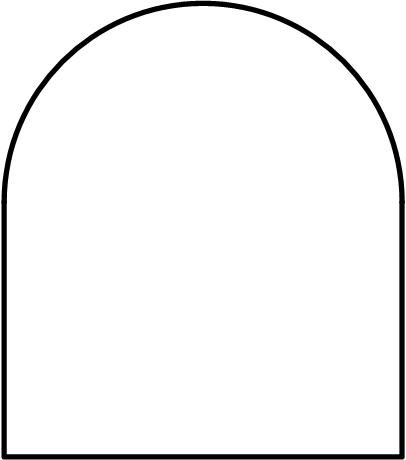
\includegraphics{./Fig/Fig07_01.PNG}} のような図形を記述したものである。
\vspc{+0.50zw}\begin{mdframed}[roundcorner=0.50zw,leftmargin=3.00zw,rightmargin=3.00zw,skipabove=0.40zw,skipbelow=0.40zw,innertopmargin=4.00pt,innerbottommargin=4.00pt,innerleftmargin=5.00pt,innerrightmargin=5.00pt,linecolor=gray!020,linewidth=0.50pt,backgroundcolor=gray!20]
\begin{verbatim}
%!PS               % PS ファイルはこの 4 文字で始まる。
10 10 moveto       % 点 (10,10) に移動する。
30 10 lineto       % 点 (30,10) まで線分を引く。
20 20 10 0 180 arc % 中心 (20,20)、半径 10、角度 0 ~ 180 度の円弧を引く。
closepath          % パスを閉じる。
stroke             % 実際に線を描く。
showpage           % ページ全体を出力する。
\end{verbatim}
\end{mdframed}\vspc{-0.70zw}
このように、PS ファイルの基本はテキストファイルである。
簡単な命令をいくつか覚えれば手で記述することもできる。
長さの単位は 1/72 である。\\

このテキストファイルを、例えば test.ps という名前で保存し、Ghostscript などの PS(互換)ソフトで開けば、先程のような図形を画面で確認することができる。
また、PS(互換)プリンタに送れば、紙に出力される。
%%
%% 項:Ghostscript
%%----------------------------------------------------------------------------------------------------------%%
\subsection{Ghostscript}
\ruby{Ghostscript}{ゴーストスクリプト} はオープンソースの PS 言語インタプリタ、すなわち PS 言語で書かれた図形を画面表示したり、一般のプリンタに出力したりするソフトウェアである。
別の言い方をすれば、Ghostscript とは PostScript 互換のソフトウェア \ruby{RIP}{リップ}(ラスタライザ)である。
RIP とは Raster Image Processor の略で、PostScript データをラスター画像(ビットマップ)に変換する装置またはソフトウェアである。
Ghostscript は PDF のラスタライズや、PostScript から PDF への変換もできる。
pdf\TeX{}や dvipdfmx などは、EPS 形式の図を出力するために Ghostscript を利用している。
%%
%% 節:EPS とは?
%%--------------------------------------------------------------------------------------------------------------------%%
\section{EPS とは?}
EPS(Encapsulated Postscript:カプセル化されたポストスクリプト)とは、1 つの図のみを含む限定された PostScript 形式のことである。
EPS ファイルのことを EPSF とも書く。
EPS ファイルは次のような行で始まる。
\vspc{+0.50zw}\begin{mdframed}[roundcorner=0.50zw,leftmargin=3.00zw,rightmargin=3.00zw,skipabove=0.40zw,skipbelow=0.40zw,innertopmargin=4.00pt,innerbottommargin=4.00pt,innerleftmargin=5.00pt,innerrightmargin=5.00pt,linecolor=gray!020,linewidth=0.50pt,backgroundcolor=gray!20]
\begin{verbatim}
%!PS-Adobe-3.0 EPSF-3.0
\end{verbatim}
\end{mdframed}\vspc{-0.70zw}
これ以降は、若干のコメント(\texttt{\%} で始まる行)と PS 言語による図形の表現が続く。\\

通常の PS ファイルは複数ページの図を含むが、EPS ファイルにはページという概念が存在しない。
また、EPS ファイルの先頭付近には「バウンディングボックス」情報が必ず付加されている。
バウンディングボックスとは図の外枠のことで、EPS ファイルの先頭付近に、
\vspc{+0.50zw}\begin{mdframed}[roundcorner=0.50zw,leftmargin=3.00zw,rightmargin=3.00zw,skipabove=0.40zw,skipbelow=0.40zw,innertopmargin=4.00pt,innerbottommargin=4.00pt,innerleftmargin=5.00pt,innerrightmargin=5.00pt,linecolor=gray!020,linewidth=0.50pt,backgroundcolor=gray!20]
\begin{verbatim}
%%BoundingBox: 12 202 571 776
\end{verbatim}
\end{mdframed}\vspc{-0.70zw}
のような形式で記述されている。
これは図の左下隅の座標が $(12,202)$、右上隅の座標が $(571,776)$ であることを意味している(単位は 1/72 インチ)。\\

EPS ファイルによっては、通常のバウンディングボックス情報以外に、
\vspc{+0.50zw}\begin{mdframed}[roundcorner=0.50zw,leftmargin=3.00zw,rightmargin=3.00zw,skipabove=0.40zw,skipbelow=0.40zw,innertopmargin=4.00pt,innerbottommargin=4.00pt,innerleftmargin=5.00pt,innerrightmargin=5.00pt,linecolor=gray!020,linewidth=0.50pt,backgroundcolor=gray!20]
\begin{verbatim}
%%HiResBoundingBox: 12.3456 201.789 570.6895 776.1234
\end{verbatim}
\end{mdframed}\vspc{-0.70zw}
のような小数点以下を含むバウンディングボックス情報を保持しているものもある。
通常、\LaTeX{}はこちらの情報を無視するが、これを読むようにするには、
\vspc{+0.50zw}\begin{mdframed}[roundcorner=0.50zw,leftmargin=3.00zw,rightmargin=3.00zw,skipabove=0.40zw,skipbelow=0.40zw,innertopmargin=4.00pt,innerbottommargin=4.00pt,innerleftmargin=5.00pt,innerrightmargin=5.00pt,linecolor=gray!020,linewidth=0.50pt,backgroundcolor=gray!20]
\begin{verbatim}
\usepackage[hiresbb]{graphicx}
\end{verbatim}
\end{mdframed}\vspc{-0.70zw}
あるいは、個々の図を読み込むところで、
\vspc{+0.50zw}\begin{mdframed}[roundcorner=0.50zw,leftmargin=3.00zw,rightmargin=3.00zw,skipabove=0.40zw,skipbelow=0.40zw,innertopmargin=4.00pt,innerbottommargin=4.00pt,innerleftmargin=5.00pt,innerrightmargin=5.00pt,linecolor=gray!020,linewidth=0.50pt,backgroundcolor=gray!20]
\begin{verbatim}
\includegraphics[hiresbb,width=5cm]{sample.eps}
\end{verbatim}
\end{mdframed}\vspc{-0.70zw}
のように hiresbb オプションを付加する。\\

\LaTeX{}は EPS ファイルの中の図を解釈することはしない。
単にバウンディングボックス情報だけを見て、確保する大きさを決定する。
%%
%% 節:PDF とは?
%%--------------------------------------------------------------------------------------------------------------------%%
\section{PDF とは?}
PDF(Portable Document Format)とは、PostScript と同じ Adobe Systems が開発したオープンな文書フォーマットである。
PostScript の進化形とも言われるので、インターネットでの情報交換から印刷所への入稿まで、広く用いられている。
Adobe から無償で配布されている Reader\footnote{最初は Acrobat Reader という名前だったが、Adobe Reader に改称され、現在は Adobe Acrobat Reader DC という名前になった。より高機能な Adobe Acrobat とは別物である。} をはじめ、多くの PDF 閲覧ソフトが存在する。\\

PDF にすればどんな環境でも同じ出力ができるというのが理想だが、現実にはフォント環境が異なれば出力も異なってしまう。
これを避けるために、PDF には使用した文字のフォントデータを埋め込むことができる。
%%
%% 節:SVG とは?
%%--------------------------------------------------------------------------------------------------------------------%%
\section{SVG とは?}
SVG(Scalable Vector Graphics)は XML ベースの新しいベクトル形式の画像フォーマットである。
最近のブラウザは SVG 画像に対応している。
Adobe Illustrator やオープンソースの Inkscape などで作成することができる他、テキストファイルなので手で書くこともできる。
例えば、
\vspc{+0.50zw}\begin{mdframed}[roundcorner=0.50zw,leftmargin=3.00zw,rightmargin=3.00zw,skipabove=0.40zw,skipbelow=0.40zw,innertopmargin=4.00pt,innerbottommargin=4.00pt,innerleftmargin=5.00pt,innerrightmargin=5.00pt,linecolor=gray!020,linewidth=0.50pt,backgroundcolor=gray!20]
\begin{verbatim}
<svg xmlns="http://www.w3.org/2000/svg" version="1.1"
     width="50" height="50" style="font-size:16px">
  <circle cx="25" cy="25" r="22" fill="#CCCCCC"
          stroke="black" stroke-width="2" />
  <text x="25" y="30" text-anchor="middle">まる</text>
</svg>
\end{verbatim}
\end{mdframed}\vspc{-0.70zw}
と記述したテキストファイルを maru.svg という名前で保存し、ブラウザで開けば \raisebox{-4.00pt}{\scalebox{0.30}{
\includegraphics{./Fig/Fig07_02.PNG}}} のような画像が表示される。\\

\LaTeX{}で使うには、予め Inckscape などのツールで PDF に変換するのが簡単である。\enlargethispage{+0.10zw}
Inkscape には「PDF+LaTeX: Omit text in PDF, and create LaTeX file」という保存方法が存在し、SVG からテキストを除いたものを maru.pdf、テキスト部分を\LaTeX{}形式で maru.pdf\_tex というファイル名で出力する。\\

これらを統合して出力するには、プリアンブルで svg パッケージを読み込んでおき、図を出力したいところに \verb`\includesvg{maru}` と記述する。
Inkscape が inkscape コマンドで呼び出せるように設定された環境では、\LaTeX{}を \verb`--shell-escape` オプション付きで起動すれば、変換まで自動で行ってくれる。
%%
%% 節:文字列の変形
%%--------------------------------------------------------------------------------------------------------------------%%
\section{文字列の変形}
graphicx パッケージを使うと、\verb`\includegraphics` 以外にもいろいろなコマンドが使えるようになる。
特に便利な文字列変形のコマンド群を挙げておく。
%%
%% 項:\rotatebox[オプション]{角度}{文字列}
%%----------------------------------------------------------------------------------------------------------%%
\subsection{\texttt{$\backslash$rotatebox[\textcolor{blue}{オプション}]\{\textcolor{blue}{角度}\}\{\textcolor{blue}{文字列}\}}}
文字列を回転する。
\vspc{-1.50zw}\begin{longtable}[l]{@{}lcl@{}}
  \hspc{+1.00zw}\verb`文字列を\rotatebox{45}{傾けて}書くことができる。` & → & \hspc{+1.00zw}文字列を\rotatebox{45}{傾けて}書くことができる。
\end{longtable}\vspc{-0.50zw}
オプション \texttt{[origin=c]} を指定すると、文字列の中心が回転の中心となる。
\texttt{[origin=tr]} なら、文字列の右上隅が回転の中心となる。
\texttt{origin} 指定で使用できるのは \texttt{lrctbB}(それぞれ左、右、中、上、下、ベースライン)とその 2 文字の組み合わせである。
回転の中心は \texttt{[x=3mm,y=2mm]} のように座標で指定することもできる。
無指定では回転の単位は度だが、\texttt{[units=6.2832]} でラジアンに変更することができる。
%%
%% 項:\scalebox{倍率}[縦の倍率]{文字列}
%%----------------------------------------------------------------------------------------------------------%%
\subsection{\texttt{$\backslash$scalebox\{\textcolor{blue}{倍率}\}[\textcolor{blue}{縦の倍率}]\{\textcolor{blue}{文字列}\}}}
文字を拡大縮小する。
オプションの縦の倍率を指定しなければ、縦も横も同じ倍率で拡大縮小される。\\

半角\scalebox{0.5}[1]{カナ}は \verb`\scalebox{0.5}[1]{カナ}` のように書くことができる。
倍角ダッシュ\scalebox{2}[1]{―}は \verb`\scalebox{2}[1]{―}` のように書くことができる。
%%
%% 項:\reflectbox{文字列}
%%----------------------------------------------------------------------------------------------------------%%
\subsection{\texttt{$\backslash$reflectbox\{\textcolor{blue}{文字列}\}}}
文字列を\reflectbox{鏡像反転}する。
\verb`\scalebox{-1}[1]{文字列}` と同じである。
%%
%% 項:\resizebox{幅}{高さ}{文字列}
%%----------------------------------------------------------------------------------------------------------%%
\subsection{\texttt{$\backslash$resizebox\{\textcolor{blue}{幅}\}\{\textcolor{blue}{高さ}\}\{\textcolor{blue}{文字列}\}}}
文字列を指定の幅・高さに拡大縮小する。
\verb`\resizebox*` のように \verb`*` を付けると「高さ」が「高さ+深さ」になる。
幅と高さを同じ倍率で拡大縮小するには、一方の長さだけを指定して、もう一方を \verb`!` とする。
元々の幅は \verb`\width`、高さは \verb`\height` と書く。\\

長い数式をページに押し込みたい場合にも使うことができる。
次の例では、数式の幅を行長(\verb`\columnwidth`)の 0.9 倍にしている。
\vspc{+0.50zw}\begin{mdframed}[roundcorner=0.50zw,leftmargin=3.00zw,rightmargin=3.00zw,skipabove=0.40zw,skipbelow=0.40zw,innertopmargin=4.00pt,innerbottommargin=4.00pt,innerleftmargin=5.00pt,innerrightmargin=5.00pt,linecolor=gray!020,linewidth=0.50pt,backgroundcolor=gray!20]
\begin{verbatim}
\resizebox{0.9\columnwidth}{!}
          {$\displaystyle \kappa = \kappa_{1} + \kappa_{2} + \frac{...}{D}$}
\end{verbatim}
\end{mdframed}\vspc{-1.70zw}
%%
%% 節:色空間とその変換
%%--------------------------------------------------------------------------------------------------------------------%%
\section{色空間とその変換}
パソコンの画面の色は光の 3 原色の赤・緑・青(Red、Green、Blue:合わせて RGB と呼ぶ)で作られている。
これに対して、印刷で使うプロセスカラーはシアン、マゼンタ、イエロー、ブラック(Cyan、Magenta、Yellow、black:合わせて CMYK と呼ぶ)を用いる。\\

原理的には CMY のみでいいはずなのだが、この 3 色を混ぜて完全な黒を表すのは難しいだけでなく、黒は文字色に使われ、CMY の黒では版が少しでもずれると文字が読みにくくなるため、黒だけは特別扱いしている。
図版では「より黒い黒」を表現するために K に CMY を被せることもある。
これ以外にも、特定の色を正確に表したい場合には、特色(スポットカラー)を用いることがある。\\

RGB と言っても、広く用いられている sRGB 以外に、より広い色域の Adobe RGB など数種類の色空間が存在する。
デジカメのカラー印刷用データには Adobe RGB を用いるべきだが、それでも CMYK の色域とは完全に一致せず、変換は単純ではない。\\

RGB データをそのまま入稿することができる仕組みが整い始めているが、今のところ印刷所に入稿する際には CMYK 対応ソフトで色合いを調整して CMYK 形式(モノクロならグレイスケール形式)で保存する方が安全である。\\

CMYK を扱えるソフトには Adobe 社の Photoshop(ラスター画像用)やIllustrator(ベクトル画像用)、オープンソースの KOffice の Krita(ラスター画像用)などが存在する。
GIMP は separete+ プラグインにより CMYK が扱えるようになる。\\

機械的な変換で構わなければ、ImageMagic の画像変換コマンド magic が便利である。
PNG 画像をグレイスケールや CMYK に変換するためのいくつかの例を以下に示す。
\vspc{+0.50zw}\begin{mdframed}[roundcorner=0.50zw,leftmargin=3.00zw,rightmargin=3.00zw,skipabove=0.40zw,skipbelow=0.40zw,innertopmargin=4.00pt,innerbottommargin=4.00pt,innerleftmargin=5.00pt,innerrightmargin=5.00pt,linecolor=gray!090,linewidth=0.50pt,backgroundcolor=gray!90]\color{gray!10}
\begin{verbatim}
$ magick foo.png -colorspace Gray foo-gray.png
$ magick foo.png -colorspace Gray EPDF:foo-gray.pdf
$ magick foo.png -colorspace CMYK EPDF:foo-cmyk.pdf
\end{verbatim}
\end{mdframed}\vspc{-0.70zw}
PDF 変換時の \texttt{EPDF:} という指定は、いわゆる Encapsulated PDF(MediaBox が用紙全体ではなく画像だけを指す PDF)にするためのものである。
ImageMagick で扱えるのはラスター画像のみで、ベクトル画像の色変換は Adobe Illustrator などを用いることになる。
%%
%% 節:色の指定
%%--------------------------------------------------------------------------------------------------------------------%%
\section{色の指定}
\LaTeX{}で色を使うには、古くは color パッケージが使われていが、ここではより強力な xcolor パッケージを紹介する。
例えば、dvipdfmx で graphics と xcolor を使うには、次のようにする。
\vspc{+0.50zw}\begin{mdframed}[roundcorner=0.50zw,leftmargin=3.00zw,rightmargin=3.00zw,skipabove=0.40zw,skipbelow=0.40zw,innertopmargin=4.00pt,innerbottommargin=4.00pt,innerleftmargin=5.00pt,innerrightmargin=5.00pt,linecolor=gray!020,linewidth=0.50pt,backgroundcolor=gray!20]
\begin{verbatim}
\documentclass[dvipdfmx]{jsarticle}
\usepackage{graphicx,xcolor}
\end{verbatim}
\end{mdframed}\vspc{-0.70zw}
色の指定は次のように行う。
\begin{itemize}
\item グレイスケールの指定は、
  \begin{quote} \verb`{\color[gray]{0.5} 文字}`\hspc{+1.00zw} 又は \hspc{+1.00zw}\verb`\textcolor[gray]{0.5}{文字}` \end{quote}
  のようにする。数値は 0 ~ 1 で、0 が黒、1 が白である。
\item カラーの印刷物なら CMYK で指定する。例えば、シアン 0.75、マゼンタ 0、Yellow 0.65、Black 0 で作る色(CUD 推奨配色の緑色)で文字を書く場合は、
  \begin{quote} \verb`{\color[cmyk]{0.75,0,0.65,0} 文字}` \hspc{+1.00zw} 又は \hspc{+1.00zw}\verb`\textcolor[cmyk]{0.75,0,0.65,0}{文字}` \end{quote}
  のようにする。
\item ディスプレイに表示する色は RGB 値で、
  \begin{quote} \verb`{\color[rgb]{0.2,0.6,0.4} 文字}`\hspc{+1.00zw} 又は \hspc{+1.00zw}\verb`\textcolor[rgb]{0.2,0.6,0.4}{文字}` \end{quote}
  のように指定する。あるいは、HTML にならった記法
  \begin{quote} \verb`{\color[HTML]{35A16B} 文字}`\hspc{+1.00zw} 又は \hspc{+1.00zw}\verb`\textcolor[HTML]{35A16B}{文字}` \end{quote}
  のように指定することもできる。
\end{itemize}
成分の割合で指定するのは面倒なので、いくつかの色名が定義されてる。
次の色はどんなドライバでも使用可能である。
\vspc{-0.50zw}\begin{description}
\setlength{\leftskip}{1.00zw}
\item[\texttt{RGB}\hspc{+0.80zw}系] red (1,0,0)、green (0,1,0)、blue (0,0,1)、brown (.75,.5,.25)、lime (.75,1,0)、orenge (1,.5,0)、pink (1,.75,.75) \\ \hspc{+12.0pt} purple (.75,0,.25)、teal (0,.5,.5)、violet (.5,0,.5)
\item[\texttt{CMYK}系] cyan (1,0,0,0)、magenta (0,1,0,0)、yellow (0,0,1,0)、olive (0.0.1,.5)
\item[\texttt{GRAY}系] black (0)、darkgray (.25)、gray (.5)、lightgray (.75)、white (1)
\end{description}\vspc{-0.50zw}
更に、black!20 で黒 20\,\%(薄い灰色)、red!30!yellow で赤 30\,\%・黄 70\,\%(赤みがかった黄)といった指定ができる。\\

\verb`\pagecolor{`\texttt{\textcolor{blue}{色の名前}}\verb`}` でページの背景色を変えることができる。
\verb`\color` 命令同様、グレイレベルや RGB、CMYK の数値でも指定可能である。
別の色を指定するまではページ色は変わったままなので、元の白に戻すには \verb`\pagecolor{white}` とする。\\

\verb`\colorbox{`\texttt{\textcolor{blue}{色名}}\verb`}{`\texttt{\textcolor{blue}{文字}}\verb`}` で文字の背景に色を付けることができる。
色は数値でも指定可能である。
\vspc{-0.50zw}\begin{longtable}[l]{@{}lcl@{}}
  \hspc{+1.00zw}\verb`\colorbox[gray]{0.8}{灰色の背景}` & → & \colorbox[gray]{0.8}{灰色の背景}
\end{longtable}\vspc{-0.50zw}
\verb`\fcolorbox{`\texttt{\textcolor{blue}{色名1}}\verb`}{`\texttt{\textcolor{blue}{色名2}}\verb`}{`\texttt{\textcolor{blue}{文字}}\verb`}` で色名 1 の枠、色名 2 の背景で文字を書くことができる。
色は数値でも指定可能である。
\vspc{-0.50zw}\begin{longtable}[l]{@{}lcl@{}}
  \hspc{+1.00zw}\verb`\fcolorbox[gray]{0}{0.8}{黒枠、灰色の背景}` & → & \fcolorbox[gray]{0}{0.8}{黒枠、灰色の背景}
\end{longtable}\vspc{-0.50zw}
%%
%% 節:枠組み
%%--------------------------------------------------------------------------------------------------------------------%%
\section{枠組み}
枠で囲む方法はさまざま存在するが、ここでは最新・最強の tcolorbox パッケージを紹介する。
このパッケージの特徴は、枠組みの途中で改ページすることができることと、多数のオプションにより多様な枠が描けることである。
内部で Ti\textit{k}Z を呼び出して使用する。\\

tcolorbox パッケージを使うには、プリアンブルに次のように記述しておく。
\vspc{+0.50zw}\begin{mdframed}[roundcorner=0.50zw,leftmargin=3.00zw,rightmargin=3.00zw,skipabove=0.40zw,skipbelow=0.40zw,innertopmargin=4.00pt,innerbottommargin=4.00pt,innerleftmargin=5.00pt,innerrightmargin=5.00pt,linecolor=gray!020,linewidth=0.50pt,backgroundcolor=gray!20]
\begin{verbatim}
\documentclass[dvipdfmx]{jsarticle}
\usepackage{tcolorbox}
\end{verbatim}
\end{mdframed}\vspc{-0.70zw}
枠組みは \verb`\begin{tcolorbox} ... \end{tcolorbox}` で行う。
次の例のように、さまざまなオプションを指定することができる。
\vspc{+0.50zw}\begin{mdframed}[roundcorner=0.50zw,leftmargin=3.00zw,rightmargin=3.00zw,skipabove=0.40zw,skipbelow=0.40zw,innertopmargin=4.00pt,innerbottommargin=4.00pt,innerleftmargin=5.00pt,innerrightmargin=5.00pt,linecolor=gray!020,linewidth=0.50pt,backgroundcolor=gray!20]
\begin{verbatim}
\begin{tcolorbox}[colframe=black!50,colback=white,colbacktitle=black!50,
                  coltitle=white,fonttitle=\bfseries\sffamily,title=粋な枠]
  わくわくする枠
\end{tcolorbox}
\end{verbatim}
\end{mdframed}\vspc{-0.70zw}
出力は次のようになる。
\vspc{+0.50zw}\begin{mdframed}[roundcorner=0.50zw,leftmargin=3.00zw,rightmargin=3.00zw,skipabove=0.40zw,skipbelow=0.40zw,innertopmargin=4.00pt,innerbottommargin=4.00pt,innerleftmargin=5.00pt,innerrightmargin=5.00pt,linecolor=gray!100,linewidth=0.50pt,backgroundcolor=gray!00]
\begin{tcolorbox}[colframe=black!50,colback=white,colbacktitle=black!50,coltitle=white,fonttitle=\bfseries\sffamily,title=粋な枠]
  わくわくする枠
\end{tcolorbox}
\end{mdframed}\vspc{-0.70zw}
